% Standalone TikZ architecture diagram of the 4-Tier Sone Neuro-Symbolic Family
\documentclass[tikz,border=5pt]{standalone}
\usepackage[T1]{fontenc}
\usepackage{lmodern}
\usepackage{amsmath,amssymb}
\usetikzlibrary{positioning,arrows.meta,fit,calc,backgrounds}
\begin{document}
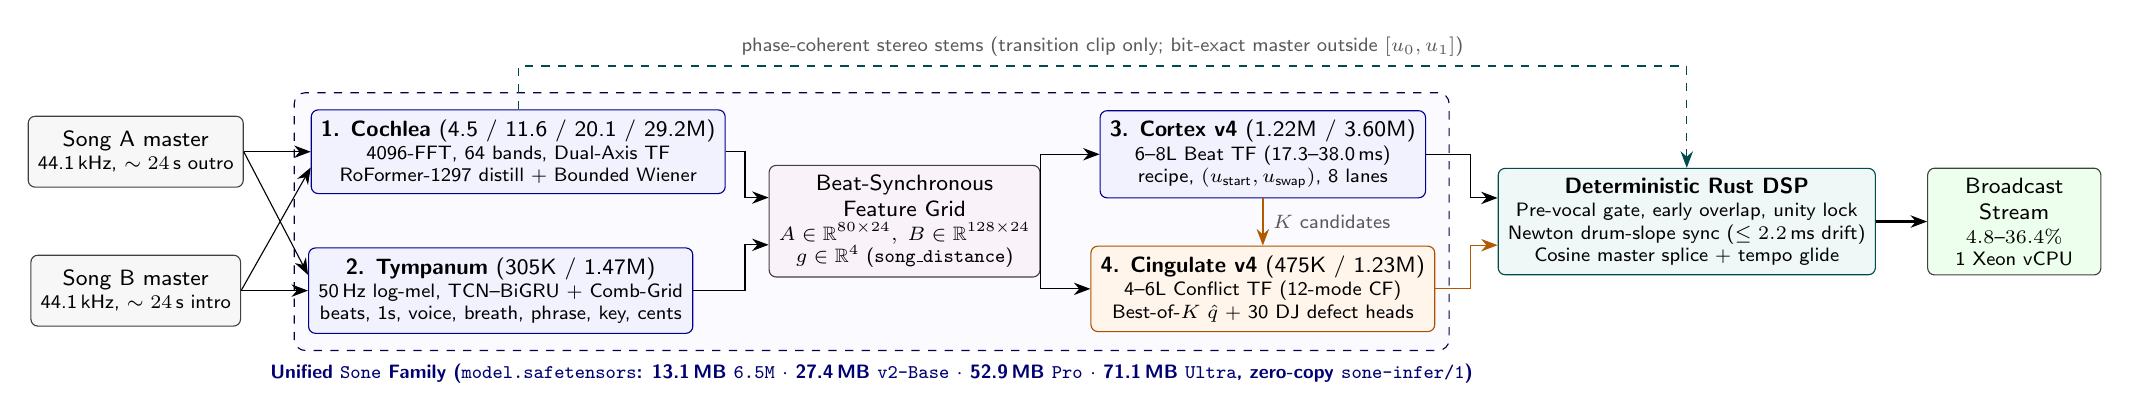
\begin{tikzpicture}[
  font=\sffamily\footnotesize,
  >={Stealth[length=2.1mm]},
  blk/.style={draw=black!75, rounded corners=2.5pt, minimum height=9mm, inner sep=3.5pt, align=center, fill=white},
  net/.style={draw=blue!55!black, rounded corners=2.5pt, minimum height=10.5mm, inner sep=3.5pt, align=center, fill=blue!5},
  dsp/.style={draw=teal!60!black, rounded corners=2.5pt, minimum height=10.5mm, inner sep=3.5pt, align=center, fill=teal!6},
  crit/.style={draw=orange!65!black, rounded corners=2.5pt, minimum height=10mm, inner sep=3.5pt, align=center, fill=orange!8},
  lab/.style={font=\sffamily\scriptsize, text=black!65},
]

% Raw inputs
\node[blk, fill=black!3, minimum width=25mm] (rawA) {Song A master\\[-1pt]\scriptsize 44.1\,kHz, $\sim 24$\,s outro};
\node[blk, fill=black!3, minimum width=25mm, below=8.5mm of rawA] (rawB) {Song B master\\[-1pt]\scriptsize 44.1\,kHz, $\sim 24$\,s intro};

% Auditory organs: Cochlea & Tympanum
\node[net, right=8.5mm of rawA, minimum width=38mm] (cochlea) {\textbf{1. Cochlea} (4.5 / 11.6 / 20.1 / 29.2M)\\[-1pt]\scriptsize 4096-FFT, 64 bands, Dual-Axis TF\\[-1.5pt]\scriptsize RoFormer-1297 distill + Bounded Wiener};
\node[net, right=8.5mm of rawB, minimum width=38mm] (tympanum) {\textbf{2. Tympanum} (305K / 1.47M)\\[-1pt]\scriptsize 50\,Hz log-mel, TCN--BiGRU + Comb-Grid\\[-1.5pt]\scriptsize beats, 1s, voice, breath, phrase, key, cents};

\draw[->] (rawA.east) -- (cochlea.west);
\draw[->] (rawB.east) -- ($(cochlea.west)+(0,-2mm)$);
\draw[->] (rawA.east) -- ($(tympanum.west)+(0,2mm)$);
\draw[->] (rawB.east) -- (tympanum.west);

% Beat-synchronous grid
\node[blk, right=7.5mm of $(cochlea.east)!0.5!(tympanum.east)$, minimum width=27mm, fill=violet!5] (grid) {Beat-Synchronous\\Feature Grid\\[-1pt]\scriptsize $A \in \mathbb{R}^{80\times24},\; B \in \mathbb{R}^{128\times24}$\\[-1.5pt]\scriptsize $g \in \mathbb{R}^4$ (\texttt{song\_distance})};

\draw[->] (cochlea.east) -| ($(grid.west)+(-3mm,3mm)$) -- ($(grid.west)+(0,3mm)$);
\draw[->] (tympanum.east) -| ($(grid.west)+(-3mm,-3mm)$) -- ($(grid.west)+(0,-3mm)$);

% Cortical stages: Cortex & Cingulate
\node[net, right=7.5mm of grid, yshift=8.5mm, minimum width=36mm] (cortex) {\textbf{3. Cortex v4} (1.22M / 3.60M)\\[-1pt]\scriptsize 6--8L Beat TF (17.3--38.0\,ms)\\[-1.5pt]\scriptsize recipe, $(u_{\text{start}}, u_{\text{swap}})$, 8 lanes};
\node[crit, below=6mm of cortex, minimum width=36mm] (cingulate) {\textbf{4. Cingulate v4} (475K / 1.23M)\\[-1pt]\scriptsize 4--6L Conflict TF (12-mode CF)\\[-1.5pt]\scriptsize Best-of-$K$ $\hat{q}$ + 30 DJ defect heads};

\draw[->] (grid.east) |- (cortex.west);
\draw[->] (grid.east) |- (cingulate.west);
\draw[->, orange!70!black, thick] (cortex.south) -- node[lab, right] {$K$ candidates} (cingulate.north);

% Handoff + DSP
\node[dsp, right=8.5mm of $(cortex.east)!0.5!(cingulate.east)$, minimum width=38mm] (dspbox) {\textbf{Deterministic Rust DSP}\\[-1pt]\scriptsize Pre-vocal gate, early overlap, unity lock\\[-1.5pt]\scriptsize Newton drum-slope sync ($\le 2.2$\,ms drift)\\[-1.5pt]\scriptsize Cosine master splice + tempo glide};

\draw[->] (cortex.east) -| ($(dspbox.west)+(-3.5mm,3mm)$) -- ($(dspbox.west)+(0,3mm)$);
\draw[->, orange!70!black] (cingulate.east) -| ($(dspbox.west)+(-3.5mm,-3mm)$) -- ($(dspbox.west)+(0,-3mm)$);
\draw[->, teal!60!black, dashed] (cochlea.north) -- ++(0,5.5mm) -| node[lab, above, pos=0.25] {phase-coherent stereo stems (transition clip only; bit-exact master outside $[u_0,u_1]$)} (dspbox.north);

% Output
\node[blk, right=6.5mm of dspbox, fill=green!7, minimum width=22mm] (out) {Broadcast\\Stream\\[-1pt]\scriptsize $4.8$--$36.4\%$\\[-1.5pt]\scriptsize 1 Xeon vCPU};
\draw[->, thick] (dspbox.east) -- (out.west);

\begin{scope}[on background layer]
  \node[draw=blue!30!black, dashed, rounded corners=4pt, fill=blue!1.5, inner xsep=5pt, inner ysep=6pt,
        fit=(cochlea) (tympanum) (grid) (cortex) (cingulate),
        label={[font=\sffamily\scriptsize\bfseries, text=blue!45!black, yshift=-1pt]below:Unified \texttt{Sone} Family (\texttt{model.safetensors}: 13.1\,MB \texttt{6.5M} $\cdot$ 27.4\,MB \texttt{v2-Base} $\cdot$ 52.9\,MB \texttt{Pro} $\cdot$ 71.1\,MB \texttt{Ultra}, zero-copy \texttt{sone-infer/1})}] {};
\end{scope}

\end{tikzpicture}
\end{document}
